\section{Stanowisko badawcze}
\label{sec:test_stand}

Konstrukcję stanowiska badawczego uzależniono od kilku czynników:
%lista punktowana
\begin{itemize}
\item prostota budowy,
\item \textbf{powtarzalność pomiarów},
\item separacja zewnętrznych czynników mogących mieć wpływ na przebieg odpowiedzi elektrycznej,
\item możliwość wymiany modelu przetwornika (patrz: Rys.\ref{fig:test_stand}),
\item łatwa zmiana mocowania przetwornika,
\item możliwość regulacji energii i pędu wymuszenia mechanicznego w zakresie \textbf{$E = 0.24\div14.4$} oraz \textbf{$p = 0.12\div4.8$} obliczonym na podstawie zależności na pęd i energię kinetyczną z fizyki klasycznej \ref{eq:kinetic_energy}.
\end{itemize}

\begin{equation}
E_{s} = \frac{m_{s} \cdot v_{s}^2}{2}
\label{eq:kinetic_energy}
\end{equation}

\begin{equation}
p_{s} = m_{s} \cdot v_{s}
\label{eq:inertia}
\end{equation}
,gdzie: $ m_s$ - masa źródła, $v_s$ - prędkość źródła, $E_s$ - energia kinetyczna źródła, $p_s$ - pęd źródła.

Po podstawieniu danych zawartych w \ref{sec:assumptions} do zależności \ref{eq:kinetic_energy} oraz otrzymano odpowiednio:

%\begin{equation}

$$E_{smin} = \frac{m_{smin} \cdot v_{smin}^2}{2}=\frac{{0.03}\cdot4^2}{2} = {0.24} mJ$$
\\$$p_{smin} = m_{smin} \cdot v_{smin} = {0.03}\cdot 10^{-3} \cdot 4 = {0.12} \cdot 10^{-3}\frac{kg \cdot m}{s^2}$$
\\$$E_{smax} = \frac{m_{smax} \cdot v_{smax}^2}{2}=\frac{0.80\cdot6^2}{2} = 14.4 mJ$$
\\$$p_{smax} = m_{smax} \cdot v_{smax} = 0.80 \cdot 6 = 4.8 \cdot 10^{-3} \frac{kg \cdot m}{s^2}$$

%\end{equation}

\indent %akapit
Biorąc pod uwagę powyższe założenia zdecydowano o zastosowaniu napędu sprężynowego w projektowanym stanowisku. Z tego powodu rozpoczęto pracę od doboru sprężyny. Głównymi kryteriami doboru były wpółczynnik sprężystości sprężyny oraz jej długość. Na podstawie zależności \ref{eq:spring} Wybrano sprężynę o $k=0.17\frac{N}{mm}$ i długości $l=80mm$. Następnie zaprojektowano układ przedstawiony na Rys.\ref{fig:test_stand}. Element symulujący źródło impulsu mechanicznego przewidziano wykonać z drewnianej sklejki. Na zdjęciu Rys.\ref{fig:test_stand_photo} przedstawiono również realizację wspomnianego stanowiska.

\begin{equation}
E_s = E_p = k \cdot x^2
\label{eq:spring}
\end{equation}
,gdzie: $E_p$ - energia potencjalna sprężystości $k$ - współczynnik sprężystości, $x$ - odkształcenie sprężyny.


\begin{figure}[htbp]
\centering
\fbox{TUTAJ PROJEKT STANOWISKA}%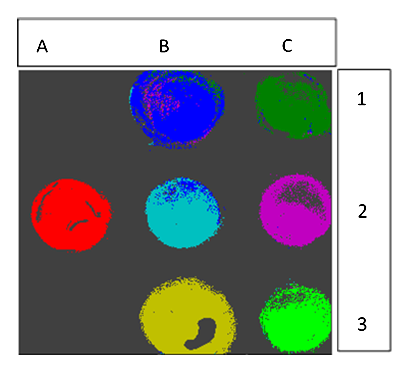
\includegraphics[width=\linewidth]{sample}}
\caption{Projekt stanowiska badawczego.}
\label{fig:test_stand}
\end{figure}

\begin{figure}[htbp]
\centering
\fbox{TUTAJ ZDJĘCIE STANOWISKA}%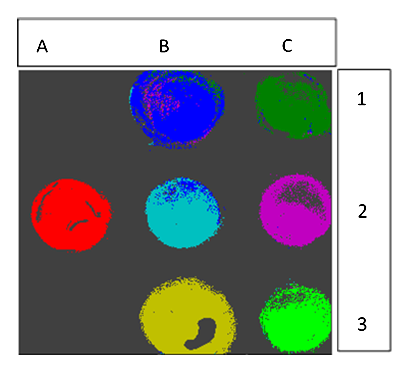
\includegraphics[width=\linewidth]{sample}}
\caption{Realizacja stanowiska badawczego.}
\label{fig:test_stand_photo}
\end{figure}